\begin{problem}{1.7}{problem1_7}

Repeat Exercise 1.6 assuming that only the angular speed \( \omega(t) \) is measured. Design a sliding mode observer to estimate the armature current, ensuring that \( \hat{i}(t) \to i(t) \) as \( t \to \infty \). Simulate the closed-loop control system with this observer. Plot the time histories of the sliding variable, the control input \( u(t) \), the angular speed \( \omega(t) \), the actual current \( i(t) \), and the estimated current \( \hat{i}(t) \).

\end{problem}

\begin{solution}{}{solution1_7}

	Let the observer estimate the state \( \hat{x}_1 \) using:
	\[
		\dot{\hat{x}}_1 = v,
	\]
	and define the observation error:
	\[
		z_1 = \hat{x}_1 - x_1.
	\]

	Taking the derivative:
	\[
		\dot{z}_1 = \dot{\hat{x}}_1 - \dot{x}_1 = v - \left(\frac{k_m}{J}x_2 - \frac{T_L}{J}\right).
	\]

	Define the correction term as:
	\[
		v = -\rho \, \text{sign}(z_1),
	\]
	with a gain satisfying:
	\[
		\rho > \frac{k_m}{J} |x_2| + \frac{|T_L|_{\max}}{J} + \beta, \quad \beta > 0.
	\]

	Thus, the observation error dynamics becomes:
	\[
		\dot{z}_1 = -\frac{k_m}{J} x_2 + \frac{T_L}{J} - \rho \, \text{sign}(z_1),
	\]
	and the Lyapunov analysis gives:
	\[
		z_1 \dot{z}_1 = z_1 \left(-\frac{k_m}{J} x_2 + \frac{T_L}{J} - \rho \, \text{sign}(z_1)\right).
	\]

	On the sliding surface \( z_1 = 0 \), the equivalent control satisfies:
	\[
		\dot{z}_1 = 0 \quad \Rightarrow \quad -\frac{k_m}{J} x_2 + \frac{T_L}{J} + v_{\text{eq}} = 0.
	\]

	Solving for \( x_2 \), we get:
	\[
		x_2 = \frac{T_L}{k_m} + \frac{J}{k_m} v_{\text{eq}}.
	\]

	Since \( T_L \) is unknown, we estimate \( x_2 \) using only \( v_{\text{eq}} \). To approximate \( v_{\text{eq}} \), we use a \emph{low-pass filter}:
	\[
		\tau \dot{\hat{v}}_{\text{eq}} = -\hat{v}_{\text{eq}} - \rho \, \text{sign}(z_1),
	\]
	where \( \tau \) is the filter time constant.\\

    And this is a great achievement, as we have now an estimate of $\dot{x}_1$, in which previously we had an unmatched disturbance. So we can redefine the sliding variable as:
    \[
        s = \dot{\hat{x}}_1 + \lambda x_1
    \]
    for the control purposes.\\

	Additionally, after the reaching time \( t_r \), we estimate:
	\[
		\hat{x}_2(t) \approx \frac{T_L}{k_m} + \frac{J}{k_m}\hat{v}_{\text{eq}}(t).
	\]

    Finally, simulating the same conditions and parameters as in Exercise 1.6, with the new sliding variable and with tho observer gain $\rho_o = 20$, and the filter time constant $\tau = 0.01$, we get the following results:

    \begin{figure}[H]
        \centering
        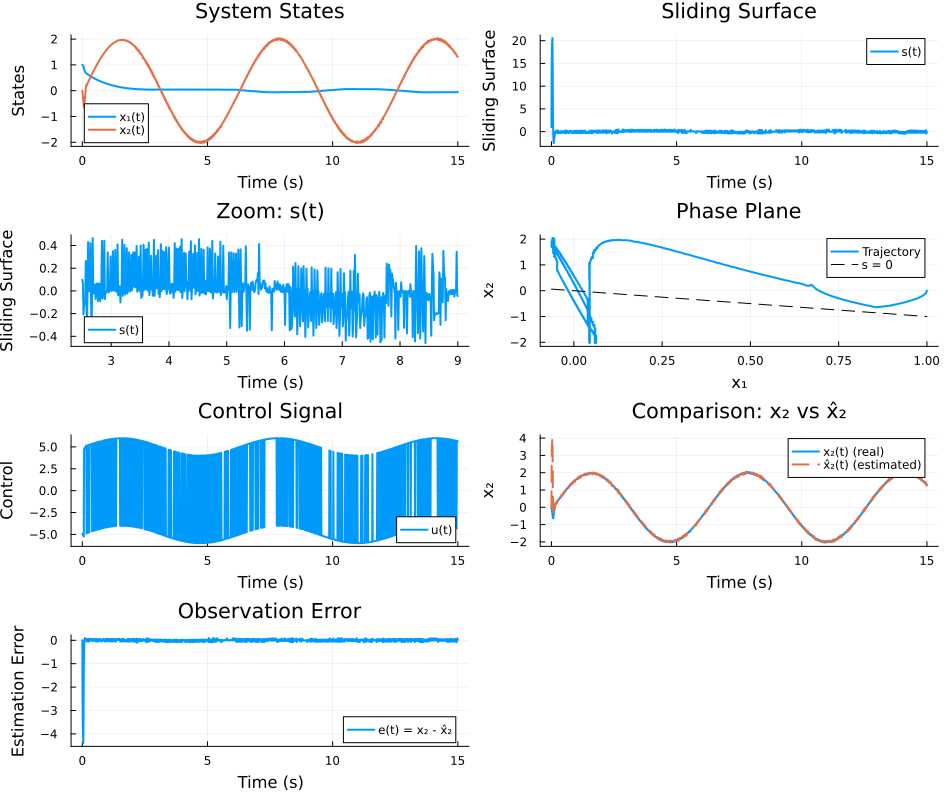
\includegraphics[width=1\textwidth]{img/problem1_7.png}
        \caption{Simulation results for the sliding mode control system with observer.}
        \label{fig:problem1_7}
    \end{figure}

    In the simulation, we observe that the sliding mode observer successfully estimates the armature current \( i(t) \), and the new sliding variable \( s(t) \) converges to zero. A key advantage of this observer is its ability to estimate the state variable \( \dot{x}_1 \), which is crucial for defining the \textit{new} sliding surface. This represents a significant improvement over the previous exercise, where we had to contend with an unmatched disturbance. Now, by effectively \textit{observing} that disturbance through the observer, we are able to compensate for it. The simulation results confirm the convergence of the angular speed \( x_1 = \omega \) to zero, fulfilling the original control objective.

\end{solution}